\documentclass{article}
\usepackage{fullpage,amssymb,amsmath,epsf}
\usepackage[12pt]{extsizes}
\usepackage{psfrag}
\usepackage{graphicx}
\usepackage{enumerate}

\newcommand{\loss}{\mathsf{L}}


\documentclass{article}
\usepackage[top = 1.0in]{geometry}

\usepackage{graphicx}

\usepackage[utf8]{inputenc}
\usepackage{listings}
\usepackage[dvipsnames]{xcolor}
\usepackage{bm}
\usepackage{algorithm}
\usepackage{algpseudocode}
\usepackage{framed}

\definecolor{codegreen}{rgb}{0,0.6,0}
\definecolor{codegray}{rgb}{0.5,0.5,0.5}
\definecolor{codepurple}{rgb}{0.58,0,0.82}
\definecolor{backcolour}{rgb}{0.95,0.95,0.92}

\lstdefinestyle{mystyle}{
    backgroundcolor=\color{backcolour},   
    commentstyle=\color{codegreen},
    keywordstyle=\color{magenta},
    stringstyle=\color{codepurple},
    basicstyle=\ttfamily\footnotesize,
    breakatwhitespace=false,         
    breaklines=true,                 
    captionpos=b,                    
    keepspaces=true,                 
    numbersep=5pt,                  
    showspaces=false,                
    showstringspaces=false,
    showtabs=false,                  
    tabsize=2
}

\lstset{style=mystyle}

\newcommand{\di}{{d}}
\newcommand{\nexp}{{n}}
\newcommand{\nf}{{p}}
\newcommand{\vcd}{{\textbf{D}}}
\newcommand{\Int}{\mathbb{Z}}
\newcommand\bb{\ensuremath{\mathbf{b}}}
\newcommand\bs{\ensuremath{\mathbf{s}}}
\newcommand\bp{\ensuremath{\mathbf{p}}}
\newcommand{\relu} { \operatorname{ReLU} }
\newcommand{\smx} { \operatorname{softmax} }
\newcommand\bx{\ensuremath{\mathbf{x}}}
\newcommand\bh{\ensuremath{\mathbf{h}}}
\newcommand\bc{\ensuremath{\mathbf{c}}}
\newcommand\bW{\ensuremath{\mathbf{W}}}
\newcommand\by{\ensuremath{\mathbf{y}}}
\newcommand\bo{\ensuremath{\mathbf{o}}}
\newcommand\be{\ensuremath{\mathbf{e}}}
\newcommand\ba{\ensuremath{\mathbf{a}}}
\newcommand\bu{\ensuremath{\mathbf{u}}}
\newcommand\bv{\ensuremath{\mathbf{v}}}
\newcommand\bP{\ensuremath{\mathbf{P}}}
\newcommand\bg{\ensuremath{\mathbf{g}}}
\newcommand\bX{\ensuremath{\mathbf{X}}}
% real numbers R symbol
\newcommand{\Real}{\mathbb{R}}

% encoder hidden
\newcommand{\henc}{\bh^{\text{enc}}}
\newcommand{\hencfw}[1]{\overrightarrow{\henc_{#1}}}
\newcommand{\hencbw}[1]{\overleftarrow{\henc_{#1}}}

% encoder cell
\newcommand{\cenc}{\bc^{\text{enc}}}
\newcommand{\cencfw}[1]{\overrightarrow{\cenc_{#1}}}
\newcommand{\cencbw}[1]{\overleftarrow{\cenc_{#1}}}

% decoder hidden
\newcommand{\hdec}{\bh^{\text{dec}}}

% decoder cell
\newcommand{\cdec}{\bc^{\text{dec}}}

\usepackage[hyperfootnotes=false]{hyperref}
\hypersetup{
  colorlinks=true,
  linkcolor = blue,
  urlcolor  = blue,
  citecolor = blue,
  anchorcolor = blue,
  pdfborderstyle={/S/U/W 1}
}
\usepackage{nccmath}
\usepackage{mathtools}
\usepackage{graphicx,caption}
\usepackage[shortlabels]{enumitem}
\usepackage{epstopdf,subcaption}
\usepackage{psfrag}
\usepackage{amsmath,amssymb,epsf}
\usepackage{verbatim}
\usepackage{cancel}
\usepackage{color,soul}
\usepackage{bbm}
\usepackage{listings}
\usepackage{setspace}
\usepackage{float}
\definecolor{Code}{rgb}{0,0,0}
\definecolor{Decorators}{rgb}{0.5,0.5,0.5}
\definecolor{Numbers}{rgb}{0.5,0,0}
\definecolor{MatchingBrackets}{rgb}{0.25,0.5,0.5}
\definecolor{Keywords}{rgb}{0,0,1}
\definecolor{self}{rgb}{0,0,0}
\definecolor{Strings}{rgb}{0,0.63,0}
\definecolor{Comments}{rgb}{0,0.63,1}
\definecolor{Backquotes}{rgb}{0,0,0}
\definecolor{Classname}{rgb}{0,0,0}
\definecolor{FunctionName}{rgb}{0,0,0}
\definecolor{Operators}{rgb}{0,0,0}
\definecolor{Background}{rgb}{0.98,0.98,0.98}
\lstdefinelanguage{Python}{
    numbers=left,
    numberstyle=\footnotesize,
    numbersep=1em,
    xleftmargin=1em,
    framextopmargin=2em,
    framexbottommargin=2em,
    showspaces=false,
    showtabs=false,
    showstringspaces=false,
    frame=l,
    tabsize=4,
    % Basic
    basicstyle=\ttfamily\footnotesize\setstretch{1},
    backgroundcolor=\color{Background},
    % Comments
    commentstyle=\color{Comments}\slshape,
    % Strings
    stringstyle=\color{Strings},
    morecomment=[s][\color{Strings}]{"""}{"""},
    morecomment=[s][\color{Strings}]{'''}{'''},
    % keywords
    morekeywords={import,from,class,def,for,while,if,is,in,elif,else,not,and,or
    ,print,break,continue,return,True,False,None,access,as,,del,except,exec
    ,finally,global,import,lambda,pass,print,raise,try,assert},
    keywordstyle={\color{Keywords}\bfseries},
    % additional keywords
    morekeywords={[2]@invariant},
    keywordstyle={[2]\color{Decorators}\slshape},
    emph={self},
    emphstyle={\color{self}\slshape},
%
}
\lstMakeShortInline|

\pagestyle{empty} \addtolength{\textwidth}{1.0in}
\addtolength{\textheight}{0.5in}
\addtolength{\oddsidemargin}{-0.5in}
\addtolength{\evensidemargin}{-0.5in}
\newcommand{\ruleskip}{\bigskip\hrule\bigskip}
\newcommand{\nodify}[1]{{\sc #1}}
\newenvironment{answer}{\sf \begingroup\color{ForestGreen}}{\endgroup}%

\setlist[itemize]{itemsep=2pt, topsep=0pt}
\setlist[enumerate]{itemsep=6pt, topsep=0pt}

\setlength{\parindent}{0pt}
\setlength{\parskip}{4pt}
\setlist[enumerate]{parsep=4pt}
\setlength{\unitlength}{1cm}

\renewcommand{\Re}{{\mathbb R}}
\newcommand{\R}{\mathbb{R}}
\newcommand{\what}[1]{\widehat{#1}}

\renewcommand{\comment}[1]{}
\newcommand{\mc}[1]{\mathcal{#1}}
\newcommand{\half}{\frac{1}{2}}

\DeclareMathOperator*{\argmin}{arg\,min}

\def\KL{D_{KL}}
\def\xsi{x^{(i)}}
\def\ysi{y^{(i)}}
\def\zsi{z^{(i)}}
\def\E{\mathbb{E}}
\def\calN{\mathcal{N}}
\def\calD{\mathcal{D}}
\def\slack{\url{http://xcs229-scpd.slack.com/}}
\def\zipscriptalt{\texttt{python zip\_submission.py}}
\DeclarePairedDelimiter\abs{\lvert}{\rvert}%
 
\usepackage{bbding}
\usepackage{pifont}
\usepackage{wasysym}
\usepackage{amssymb}
\usepackage{framed}
\usepackage{scrextend}

\newcommand{\alns}[1] {
	\begin{align*} #1 \end{align*}
}

\newcommand{\pd}[2] {
 \frac{\partial #1}{\partial #2}
}
\renewcommand{\Re} { \mathbb{R} }
\newcommand{\btx} { \mathbf{\tilde{x}} }
\newcommand{\bth} { \mathbf{\tilde{h}} }
\newcommand{\sigmoid} { \operatorname{\sigma} }
\newcommand{\CE} { \operatorname{CE} }
\newcommand{\byt} { \hat{\by} }
\newcommand{\yt} { \hat{y} }

\newcommand{\oft}[1]{^{(#1)}}
\newcommand{\fone}{\ensuremath{F_1}}

\newcommand{\ac}[1]{ {\color{red} \textbf{AC:} #1} }
\newcommand{\ner}[1]{\textbf{\color{blue} #1}}

\begin{document}
\title{XCS229 Supplemental Lecture Notes}
\author{Andrew Ng}
%\date{Lectures from 1/7/03 to 1/16/03}
\date{}
\maketitle

\section{Binary classification}

In \textbf{binary classification} problems, the target $y$ can take on at
only two values. In this set of notes, we show how to model this problem by
letting $y \in \{-1, +1\}$, where we say that $y$ is a $1$ if the example is
a member of the positive class and $y = -1$ if the example is a member of
the negative class. We assume, as usual, that we have input features
$x \in \R^n$.

As in our standard approach to supervised learning problems, we first pick a
representation for our hypothesis class (what we are trying to learn), and
after that we pick a loss function that we will minimize.  In
binary classification problems, it is often convenient to use a hypothesis
class of the form $h_\theta(x) = \theta^T x$, and, when presented
with a new example $x$, we classify it as positive or negative
depending on the sign of $\theta^T x$, that is, our predicted
label is
\begin{equation*}
  \sign(h_\theta(x)) = \sign(\theta^T x)
  ~~ \mbox{where} ~~
  \sign(t) =
  \begin{cases} 1 & \mbox{if}~ t > 0 \\
    0 & \mbox{if~} t = 0 \\
    -1 & \mbox{if~} t < 0.
  \end{cases}
\end{equation*}
In a binary classification problem, then, the hypothesis $h_\theta$
with parameter vector $\theta$ classifies a particular example
$(x, y)$ correctly if
\begin{equation}
  \label{eqn:predict-correct}
  \sign(\theta^T x) = y
  ~~~ \mbox{or equivalently} ~~~
  y \theta^T x > 0.
\end{equation}
The quantity $y \theta^T x$ in expression~\eqref{eqn:predict-correct} is a
very important quantity in binary classification, important enough that we
call the value
\begin{equation*}
  y x^T \theta
\end{equation*}
the \emph{margin} for the example $(x, y)$. Often, though not always, one
interprets the value $h_\theta(x) = x^T \theta$ as a measure of the
confidence that the parameter vector $\theta$ assigns to labels for the
point $x$: if $x^T \theta$ is very negative (or very positive), then we more
strongly believe the label $y$ is negative (or positive).

Now that we have chosen a representation for our data, we must choose a loss
function. Intuitively, we would like to choose some loss function so that
for our training data $\{(\xsi, \ysi)\}_{i = 1}^m$, the $\theta$ chosen
makes the margin $\ysi \theta^T \xsi$ very large for each training example.
Let us fix a hypothetical example $(x, y)$, let $z = y x^T \theta$ denote
the margin, and let $\loss : \R \to \R$ be the loss function---that is,
the loss for the example $(x, y)$ with margin $z = y x^T \theta$ is
$\loss(z) = \loss(y x^T \theta)$.
For any particular loss function, the empirical risk that we minimize
is then
\begin{equation}
  J(\theta)
  = \frac{1}{m} \sum_{i = 1}^m \loss(\ysi \theta^T \xsi).
\end{equation}

\newcommand{\zoloss}{\loss_{\rm zo}}
\newcommand{\logloss}{\loss_{\rm logistic}}
\newcommand{\hingeloss}{\loss_{\rm hinge}}
\newcommand{\exploss}{\loss_{\rm exp}}
\newcommand{\hinge}[1]{\left[{#1}\right]_+}

Consider our desired behavior: we wish to have $\ysi \theta^T \xsi$ positive
for each training example $i = 1, \ldots, m$, and we should penalize those
$\theta$ for which $\ysi \theta^T \xsi < 0$ frequently in the training
data. Thus, an intuitive choice for our loss would be one with $\loss(z)$
small if $z > 0$ (the margin is positive), while $\loss(z)$ is large if $z
< 0$ (the margin is negative).
Perhaps the most natural such loss is the \emph{zero-one} loss,
given by
\begin{equation*}
  \zoloss(z) = \begin{cases} 1 & \mbox{if~} z \le 0 \\
    0 & \mbox{if}~ z > 0.
  \end{cases}
\end{equation*}
In this case, the risk $J(\theta)$ is simply the average number of
mistakes---misclassifications---the parameter $\theta$ makes on the training
data. Unfortunately, the loss $\zoloss$ is discontinuous, non-convex (why
this matters is a bit beyond the scope of the course), and perhaps even more
vexingly, NP-hard to minimize. So we prefer to choose losses that have the
shape given in Figure~\ref{fig:simple-loss-shape}.
\begin{figure}[h!]
  \begin{center}
    \psfrag{varphi}{$\loss$}
    \psfrag{z = yxTtheta}{$z = y x^T \theta$}
    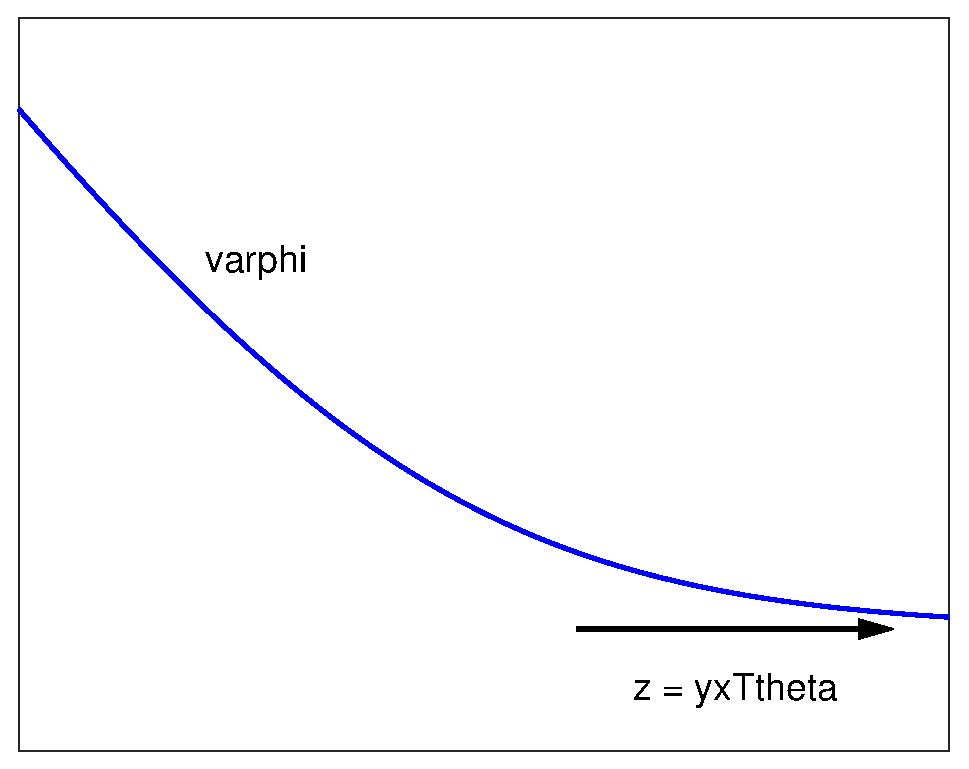
\includegraphics[width=.6\columnwidth]{logistic-loss.eps}
    \caption{\label{fig:simple-loss-shape} The rough shape
      of loss we desire: the loss is convex and continuous,
      and tends to zero as the margin $z = y x^T \theta \to \infty$.}
  \end{center}
\end{figure}
That is, we will essentially always use losses that satisfy
\begin{equation*}
  \loss(z) \to 0
  ~~ \mbox{as}~ z \to \infty,
  ~~ \mbox{while} ~~
  \loss(z) \to \infty
  ~~ \mbox{as} ~ z \to -\infty.
\end{equation*}

As a few different examples, here are three loss functions that
we will see either now or later in the class, all of which are commonly
used in machine learning.
\begin{enumerate}[(i)]
\item The \emph{logistic loss} uses
  \begin{equation*}
    \logloss(z) = \log(1 + e^{-z})
  \end{equation*}
\item The \emph{hinge loss} uses
  \begin{equation*}
    \hingeloss(z) = \hinge{1 - z}
    = \max\{1 - z, 0\}
  \end{equation*}
\item The \emph{exponential loss} uses
  \begin{equation*}
    \exploss(z) = e^{-z}.
  \end{equation*}
\end{enumerate}
In Figure~\ref{fig:loss-functions}, we plot each of these losses
against the margin $z = y x^T \theta$, noting that each goes to zero
as the margin grows, and each tends to $+\infty$ as the margin becomes
negative. The different loss functions lead to different machine
learning procedures; in particular, the logistic loss
$\logloss$ is logistic regression, the
hinge loss $\hingeloss$ gives rise to so-called \emph{support vector
machines}, and the exponential loss gives rise to the classical
version of \emph{boosting}, both of which we will explore in more depth
later in the class.

\begin{figure}[h!]
  \begin{center}
    \psfrag{Logistic}{$\logloss$}
    \psfrag{Hinge}{$\hingeloss$}
    \psfrag{Exp}{$\exploss$}
    \psfrag{z = yxTtheta}{$z = y x^T \theta$}
    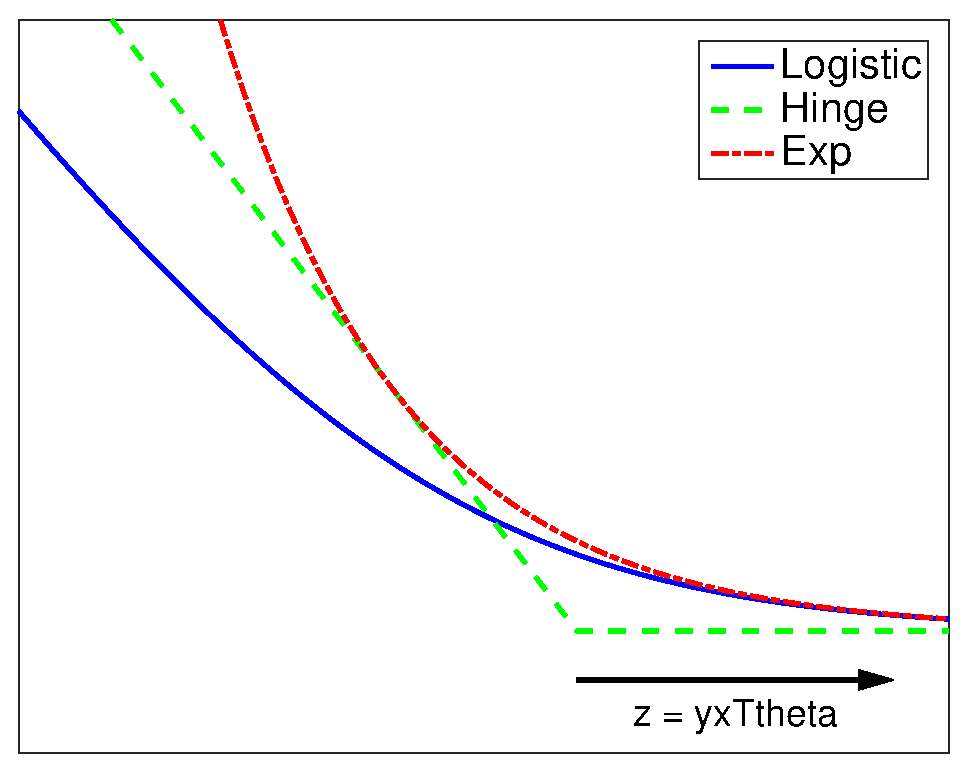
\includegraphics[width=.7\columnwidth]{many-losses.eps}
    \caption{\label{fig:loss-functions} The three margin-based loss
      functions logistic loss, hinge loss, and exponential loss.}
  \end{center}
\end{figure}

\section{Logistic regression}

With this general background in place, we now we give a complementary view
of logistic regression to that in Andrew Ng's lecture notes.
When we use binary labels $y \in \{-1, 1\}$, it is possible to
write logistic regression more compactly. In particular, we use the
logistic loss
\begin{equation*}
  \logloss(y x^T\theta)
  = \log\left(1 + \exp(-y x^T \theta)\right),
\end{equation*}
and the \emph{logistic regression} algorithm corresponds to choosing
$\theta$ that minimizes
\begin{equation}
  \label{eqn:logreg-risk}
  J(\theta) = \frac{1}{m}
  \sum_{i=1}^m \logloss(\ysi \theta^T \xsi)
  = \frac{1}{m} \sum_{i=1}^m \log\left(1 + \exp(-\ysi \theta^T \xsi)\right).
\end{equation}
Roughly, we hope that choosing $\theta$ to minimize the average logistic
loss will yield a $\theta$ for which $\ysi \theta^T \xsi > 0$ for most (or
even all!) of the training examples.


\subsection{Probabilistic intrepretation}

\begin{figure}[ht]
  \begin{center}
    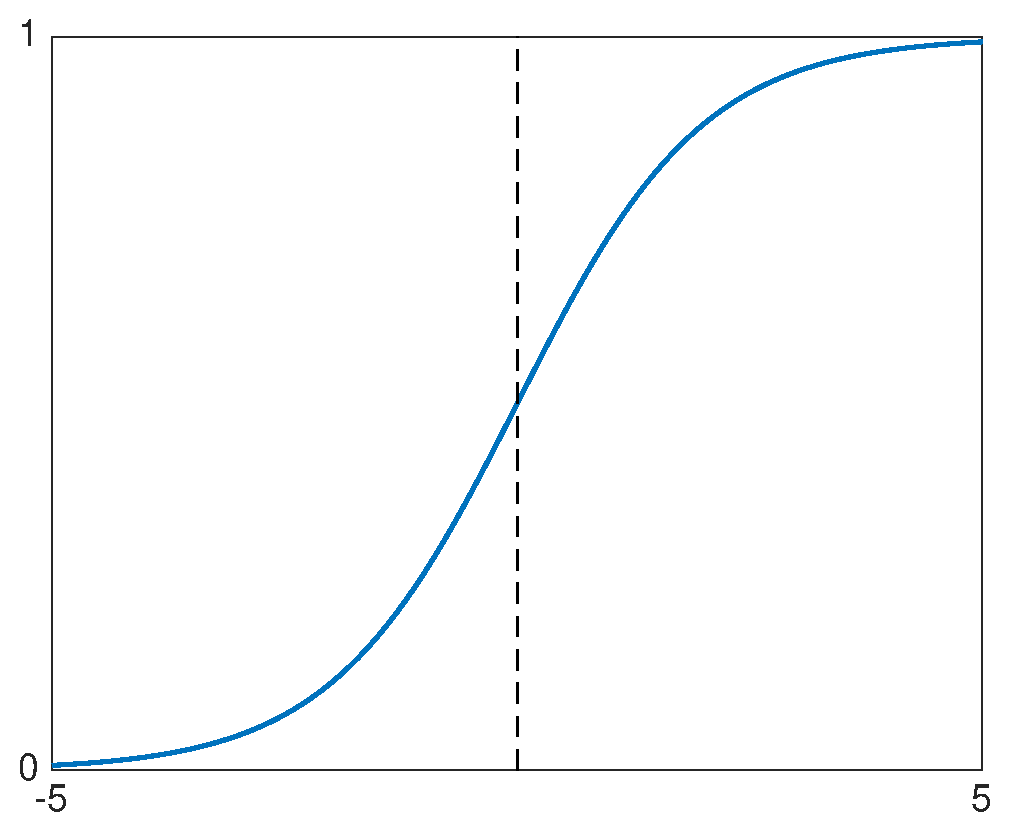
\includegraphics[width=.6\columnwidth]{sigmoid.eps}
    \caption{\label{fig:sigmoid} Sigmoid function}
  \end{center}
\end{figure}

Similar to the linear regression (least-squares) case, it
is possible to give a probabilistic interpretation of logistic
regression. To do this, we define the \emph{sigmoid function}
(also often called the \emph{logistic function})
\begin{equation*}
  g(z) = \frac{1}{1 + e^{-z}},
\end{equation*}
which is plotted in Fig.~\ref{fig:sigmoid}. In particular,
the sigmoid function satisfies
\begin{equation*}
  g(z) + g(-z) = \frac{1}{1 + e^{-z}} + \frac{1}{1 + e^z}
  = \frac{e^z}{1 + e^z} + \frac{1}{1 + e^z} = 1,
\end{equation*}
so we can use it to define a probability model for binary classification.
In particular, for $y \in \{-1, 1\}$, we define the \emph{logistic
model} for classification as
\begin{equation}
  \label{eqn:logistic-model}
  p(Y = y \mid x; \theta)
  = g(y x^T \theta)
  = \frac{1}{1 + e^{-y x^T \theta}}.
\end{equation}
For intepretation, we see that if the margin
$y x^T \theta$ is large---bigger than, say, 5 or so---then
$p(Y = y \mid x; \theta) = g(y x^T \theta) \approx 1$, that is, 
we assign nearly probability $1$ to the event that the label is $y$.
Conversely, if $y x^T \theta$ is quite negative, then
$p(Y = y \mid x; \theta) \approx 0$.

By redefining our hypothesis class as
\begin{equation*}
  h_\theta(x) = g(\theta^T x) = \frac{1}{1 + e^{-\theta^T x}},
\end{equation*}
then we see that the likelihood of the training data is
\begin{equation*}
  L(\theta)
  = \prod_{i = 1}^m p(Y = \ysi \mid \xsi; \theta)
  = \prod_{i = 1}^m h_\theta(\ysi \xsi),
\end{equation*}
and the log-likelihood is precisely
\begin{equation*}
  \ell(\theta)
  = \sum_{i = 1}^m \log h_\theta(\ysi \xsi)
  = -\sum_{i = 1}^m \log\left(1 + e^{-\ysi \theta^T \xsi}\right)
  = - m J(\theta),
\end{equation*}
where $J(\theta)$ is exactly the logistic regression
risk from Eq.~\eqref{eqn:logreg-risk}. That is, maximum likelihood
in the logistic model~\eqref{eqn:logistic-model} is the same
as minimizing the average logistic loss, and we arrive at logistic
regression again.

\subsection{Gradient descent methods}

The final part of logistic regression is to actually fit the model.
As is usually the case, we consider gradient-descent-based procedures
for performing this minimization. With that in mind, we now show
how to take derivatives of the logistic loss.
For $\logloss(z) = \log(1 + e^{-z})$,
we have the one-dimensional derivative
\begin{equation*}
  \frac{d}{dz} \logloss(z)
  = \logloss'(z)
  = \frac{1}{1 + e^{-z}} \cdot \frac{d}{dz} e^{-z}
  = -\frac{e^{-z}}{1 + e^{-z}}
  = - \frac{1}{1 + e^z} = - g(-z),
\end{equation*}
where $g$ is the sigmoid function. Then we apply the chain rule to find that
for a single training example $(x, y)$, we have
\begin{equation*}
  \frac{\partial}{\partial \theta_k}
  \logloss(y x^T \theta)
  = -g(-y x^T \theta) \frac{\partial}{\partial \theta_k} (y x^T \theta)
  = -g(-y x^T\theta) y x_k.
\end{equation*}
Thus, a stochastic gradient procedure for minimization of $J(\theta)$
iteratively performs the following for iterations
$t = 1, 2, \ldots$, where $\stepsize_t$ is a stepsize at time $t$:
\begin{enumerate}[1.]
\item Choose an example $i \in \{1, \ldots, m\}$ uniformly at random
\item Perform the gradient update
  \begin{align*}
    \theta^{(t + 1)}
    & = \theta^{(t)}
    - \stepsize_t \cdot \nabla_\theta \logloss(\ysi \xsi^T \theta^{(t)}) \\
    & = \theta^{(t)}
    + \stepsize_t
    g(-\ysi \xsi^T \theta^{(t)}) \ysi \xsi
    = \theta^{(t)}
    + \stepsize_t
    h_{\theta^{(t)}} (-\ysi \xsi) \ysi \xsi.
  \end{align*}
\end{enumerate}
This update is intuitive: if our current hypothesis
$h_{\theta^{(t)}}$ assigns probability close to $1$ for the
\emph{incorrect} label $-\ysi$, then we try to reduce the loss
by moving $\theta$ in the direction of $\ysi \xsi$. Conversely,
if our current hypothesis $h_{\theta^{(t)}}$ assigns probability
close to $0$ for the incorrect label $-\ysi$, the update essentially
does nothing.


\end{document}
